\usepackage{amsthm}

\newtheorem{theorem}{Theorem}[chapter]
\newtheorem{lemma}           [theorem] {Lemma}   
\newtheorem{folg}           [theorem] {Folgerung}   

\newtheorem{frage}       [theorem] {Frage}   
\newtheorem{question}       [theorem] {Question}   
\newtheorem{aufgabe}       [theorem] {Aufgabe}   
\newtheorem{exercise}       [theorem] {Exercise}  

\newtheorem{proposition}     [theorem] {Proposition}  
\newtheorem{satz}     [theorem] {Satz}  
\newtheorem{fact}{Fact}
\newtheorem{definition}      [theorem] {Definition} 

\theoremstyle{definition} 
\newtheorem{bemerkung}     [theorem] {Bemerkung}  
\newtheorem{beispiel}       [theorem] {Beispiel}  
\newtheorem{example}       [theorem] {Example}  
\newtheorem*{example*} {Example}  
\newtheorem{notation}       [theorem] {Notation}  
\newtheorem*{Faust}[theorem]{Rule of Thumb}
\newtheorem*{Boxx}[theorem]{Concept}

Now we present the famous mean value theorem.
\begin{Theorem}{}
Let $f:[a,b]\to\mathbb{R}$ be differentiable. Then there exists some $\hat{x}\in(a,b)$ such that
\[f(b)-f(a)=f'(\hat{x})\cdot (b-a).\]
\end{Theorem}
Before the proof is presented, we give some graphical interpretation: A~division of the above equation by $b-a$ gives
\[\frac{f(b)-f(a)}{b-a}=f'(\hat{x}).\]
The quantity on the left hand side is equal to the slope of the secant of $f$ through $a$ and $b$, whereas $f'(\hat{x})$ corresponds to the slope of tangent of $f$ at $\hat{x}$. Therefore,
the secant of $f$ through $a$ and $b$ is parallel to a tangent of $f$.

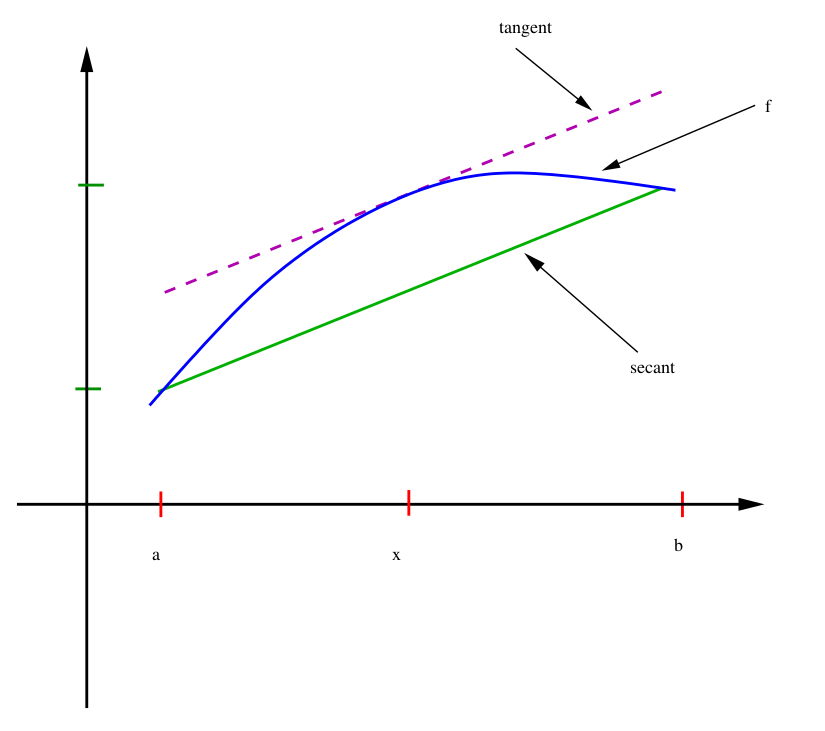
\includegraphics{./mean.png}

{\em Proof:} Consider the function $F:[a,b]\to\mathbb{R}$ with
\[F(x):=f(x)-f(a)-\frac{f(b)-f(a)}{b-a}\cdot(x-a).\]
Then we have $F(a)=F(b)=0$. By Rolle's Theorem, we get that there exists some $\hat{x}\in(a,b)$ with
\[0=F'(\hat{x})=f'(\hat{x})-\frac{f(b)-f(a)}{b-a}\]
and thus
\[f'(\hat{x})=\frac{f(b)-f(a)}{b-a}.\]
\hfill$\Box$

The mean value theorem leads us to determine monotonicity properties of a~function by means of its derivative.
\begin{Theorem}{}
    Let $f:[a,b]\to\mathbb{R}$ be a differentiable function. Then the following holds true.
\begin{enumerate}[(i)]
 \item If $f'(x)>0$ for all $x\in(a,b)$, then $f$ is strictly monotonically increasing.
 \item If $f'(x)<0$ for all $x\in(a,b)$, then $f$ is strictly monotonically decreasing.
 \item If $f'(x)\geq0$ for all $x\in(a,b)$, then $f$ is monotonically increasing.
 \item If $f'(x)\leq0$ for all $x\in(a,b)$, then $f$ is monotonically decreasing.
\end{enumerate}
\end{Theorem}
{\em Proof:}
(i) By the mean value theorem we have that for $x_1,x_2\in(a,b)$ with $x_1<x_2$, there exists some $\hat{x}\in(x_1,x_2)$ with
\[f(x_2)-f(x_1)=f'(\hat{x})\cdot(x_2-x_1)>0.\]
The results (ii)-(iv) can be proven analogously.\hfill$\Box$

